\section{Architecture}
\todo[inline]{Add some overview over what we are going to tell about the architecture through the sketches. What we mean by architecture}
In order to provide users with a all the functionality of the implementation more than a Android application was needed.
To provide statistical data and to collect data from users home a back-end was needed.

The implementation will consist of three parts. The server, The device in the users home used to 
collect and send usage data, and the Android application. The android application is the main focus for 
this project and most of the teams resources will be used on this.

\subsection{Server}
The server will consist of two parts. One for handling requests from the Android application and one for storing data that is collected in the users home. 
The part that handles the android application will be running Dropwizard~\cite{dropwizard} which is a collection of Java libraries that together make a REST service. 

These libraries include Jetty~\cite{jetty}, Jersey~\cite{jersey}, JDBC~\cite{jdbc}, and Jackson~\cite{jackson} and are discussed in further detail in the section about libraries.
The server will expose a set of URL’s that will provide the android application with 
possibilities to get and store data from the database. The other part, that stores data from the users home is under development.

\subsection{Android Application}
The application running on the users Android device will be designed to run on Android 4.0 or greater. As of March 2014 this includes 79,7\% of Android devices~\cite{androidDeviceFragmentation}. The rest is on the old Android 2.3 and above. The team decided not to include these devices since the application is a proof-of-concept, and for the purpose of the app, one can assume that the relevent users do have a modern new phone. 

The architecture will heavily rely on using ContentProviders~\cite{contentproviders} for database access. This will give a uniform access model for the data, that will not run on the UI thread. When lists of data is accesed for an Activity or a Fragment, then LoaderManagers~\cite{loadermanager} are used. This will handle the lifcecycle of data change notification through the cursor. 

The remaining problem is where to place the business logic for data manipulation. This is where the pattern Model-View-Presenter (MVP)~\cite{mvp} comes in. MVP is a Model-View-Controller (MVC)~\cite{mvc} derivative. All business logic is handled in presenter classes. Through this uniform access, all logic applied to data preservation (sever syncronization), and data control can be done. The lifecycle of the presenter classes is in the base Activity class, and all other sub fragments can get access to it though a interface. This pushes almost all logic into the presenters, making the fragments code clean.

The application will follow standard Android design guidelines~\cite{androidgui}
when it comes to user interface design.

\subsection{Home Data Aggregator}
This device will collect data from sources in the user's home. The reason for this external box as opposed to using 
the user's phone to collect data, is that with this solution the system can fetch data at regular intervals throughout 
the whole day. This would result in that the user would not need to be home in order for the application to collect 
usage data. The device will pass data along to the external server at request from the server.

\begin{figure}[H]
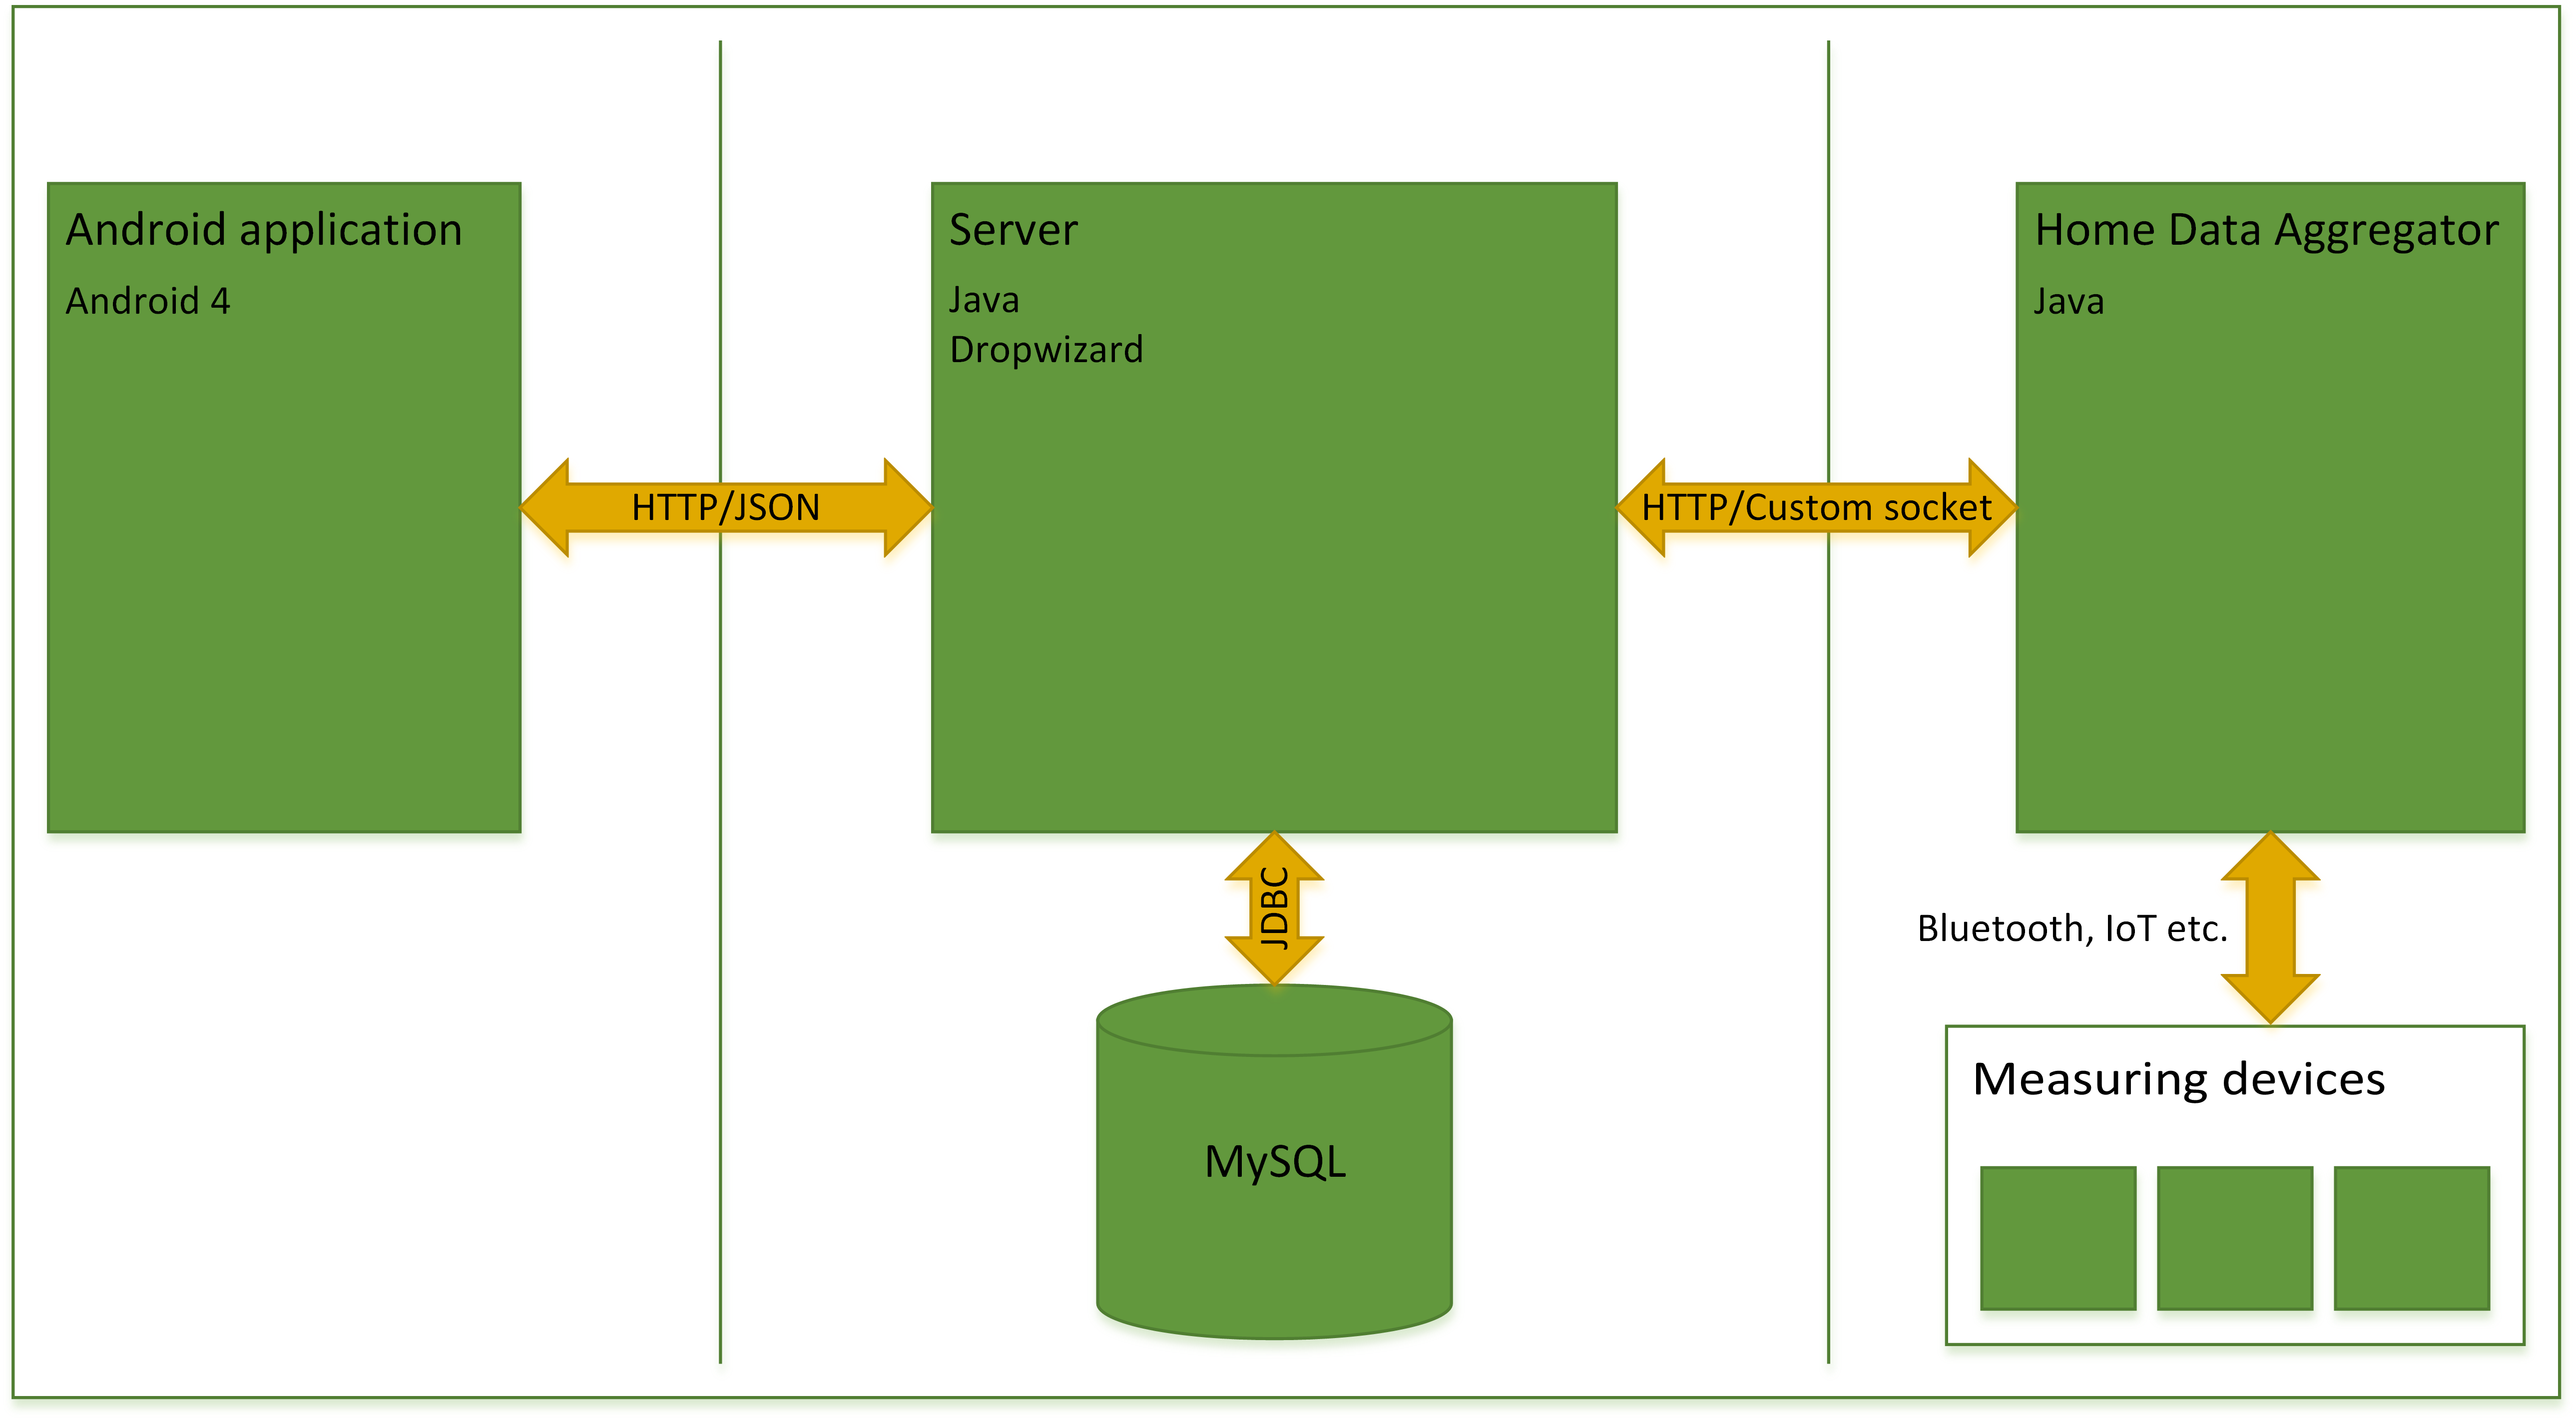
\includegraphics[width=\textwidth]{ch/implementation/fig/architecture.png}
\caption{Architecture overview}
\end{figure}